\subsection{Failure-mode taxonomy}
\label{sec:failure-taxonomy}

Aggregate AUROC obscures the structure of failure. We cluster every recording in the SPMB cohort ($n{=}276$) by its joint behavior across the canonicalized arm of the $14$ $(\text{axis},\text{severity})$ cells, yielding seven mutually exclusive failure categories.

\begin{description}\setlength{\itemsep}{1pt}
  \item[Robust-correct.] Correct at baseline and on the majority of shifted cells. The benign case.
  \item[Robust-wrong.] Wrong at baseline and stays wrong everywhere ($\leq 10\%$ shifted-cell recovery). Intrinsic classification failure; not driven by shift.
  \item[Shift-induced flip.] Correct at baseline but $\geq 30\%$ of shifted cells flip the prediction. The canonical bad pattern this paper exists to expose.
  \item[Shift-recovered.] Wrong at baseline, $\geq 60\%$ correct after shift. Suspicious: a shift that helps the model is rarely doing it for the right reason.
  \item[Calibration collapse.] Correct at baseline, retains the argmax, but $\geq 20\%$ of shifted cells land within $\pm 0.15$ of $p{=}0.5$. The model ``knows'' it is uncertain without flipping --- which a downstream selective head can catch.
  \item[Catastrophic shift.] Correct at baseline, then at least one shifted cell is wrong with $p_{\text{wrong-class}}\!\geq\!0.80$. The most clinically dangerous failure: high-confidence wrong direction under operational shift.
  \item[Axis-specific.] Correct at baseline, failures concentrated in a single axis ($\geq 50\%$ flip on one axis, $<15\%$ on the other two).
\end{description}

Table~\ref{tab:failure-counts} reports the prevalence of each category. The three most common are \emph{catastrophic shift} ($n{=}112$, 40.6\%), \emph{robust-correct} ($n{=}97$, 35.1\%), \emph{robust-wrong} ($n{=}55$, 19.9\%).

\begin{table}[t]
\centering
\caption{Failure-category prevalence on the SPMB cohort ($n{=}276$), stratified by ground-truth label.}
\label{tab:failure-counts}
\footnotesize
\begin{tabular}{lrrr}
\toprule
Category & All & Normal & Abnormal \\
\midrule
Robust-correct & 97 (35.1\%) & 0 (0.0\%) & 97 (77.0\%) \\
Shift-recovered & 3 (1.1\%) & 0 (0.0\%) & 3 (2.4\%) \\
Calibration collapse & 0 (0.0\%) & 0 (0.0\%) & 0 (0.0\%) \\
Axis-specific & 8 (2.9\%) & 4 (2.7\%) & 4 (3.2\%) \\
Shift-induced flip & 1 (0.4\%) & 1 (0.7\%) & 0 (0.0\%) \\
Catastrophic shift & 112 (40.6\%) & 102 (68.0\%) & 10 (7.9\%) \\
Robust-wrong & 55 (19.9\%) & 43 (28.7\%) & 12 (9.5\%) \\
\bottomrule
\end{tabular}
\end{table}

\paragraph{The dangerous tail.} \emph{Catastrophic shift} ($n{=}112$, 40.6\%) deserves special attention: these recordings the model classifies correctly under canonical acquisition, but at least one operational shift drives the prediction to the wrong class with confidence $\geq 0.80$. Exemplar recording \texttt{aaaaajfe\_s001\_t000} (ground truth: normal) reaches a wrong-side confidence of $0.98$ under shift. Clinically, this is the highest-priority failure mode: it produces a confident, miscalibrated report whose error signature is invisible to the clinician without a per-recording trust signal.

\paragraph{Polarized-logit signature.} The near-emptiness of the \emph{calibration-collapse} bucket ($n{=}0$) is itself a finding: the EEGPT-derived classifier does not gracefully equivocate under shift. Of the $128$ baseline-correct recordings with at least one wrong shifted cell, $112$ ($87.5\%$) are wrong with $p_{\text{wrong}}\!\geq\!0.80$. The model's logit distribution is sharply polarized; when it errs under shift it does so with full confidence. Selective heads that rely on $p\!\approx\!0.5$ as the abstention trigger will fail to catch these, motivating distributional (logit-magnitude, NP test) abstention signals.

\paragraph{Class-asymmetric vulnerability (most novel finding).} The failure load falls almost entirely on the normal class. Of $107$ baseline-correct normal recordings, \emph{every single one} flips on at least one shifted cell ($100\%$ flip incidence), and $102$ ($95.3\%$) flip with $p_{\text{abnormal}}\!\geq\!0.80$ on at least one cell --- i.e., $102/107$ baseline-correct normals are catastrophic-shift recordings. By contrast, of $111$ baseline-correct abnormals, $97$ ($87.4\%$) are robust-correct across the entire sweep, and only $10$ ($9.0\%$) are catastrophic-shift. The shift-induced failure is therefore directional: it predominantly converts a clean normal recording into a confident abnormal report. This is the worst possible direction for a screening tool, because abnormal false-positives drive the alert fatigue that drives clinician disuse. Any deployment of EEGPT-class models on non-canonical acquisition pipelines must address this normal-to-abnormal drift specifically.

\paragraph{Clinical implications by category.} Each category maps to a distinct downstream risk:
\begin{itemize}\setlength{\itemsep}{1pt}
  \item \emph{Shift-induced flip} on normal-class recordings inflates the false-alarm rate to the reading clinician; on abnormal-class recordings it produces false reassurance.
  \item \emph{Catastrophic shift} converts a quiet error into a hazardous one: the high-confidence wrong report carries the same UI weight as a correct one.
  \item \emph{Calibration collapse} is the \emph{safest} failure mode --- a selective head with a $|\,\text{logit}\,|$ threshold or NP test reliably abstains.
  \item \emph{Shift-recovered} flags a recording whose baseline answer was itself suspect; deployment should ignore the recovery and treat the baseline as authoritative.
  \item \emph{Axis-specific} failures localize blame to a single acquisition variable, enabling targeted device-side fixes (resampling kernel, gain calibration, notch filter).
\end{itemize}

\paragraph{Axis vulnerability.} Ranking the three acquisition axes by a composite of mean flip rate, mean ground-truth-class confidence drop, and $\Delta$AUROC at each axis's worst severity (canonicalized arm) places \emph{sampling\_rate} first --- $\Delta\text{AUROC}{=}0.150$, mean flip rate $0.43$, mean GT-class confidence drop $+0.23$ at severity $512$. Sampling rate dominates because non-integer resampling alters the spectral content the EEGPT backbone uses; the other axes degrade probability quality without always reorganizing the spectral evidence.

Figure~\ref{fig:failure-taxonomy} renders the per-cell composition of these categories across the full acquisition sweep.

\begin{figure}[t]
  \centering
  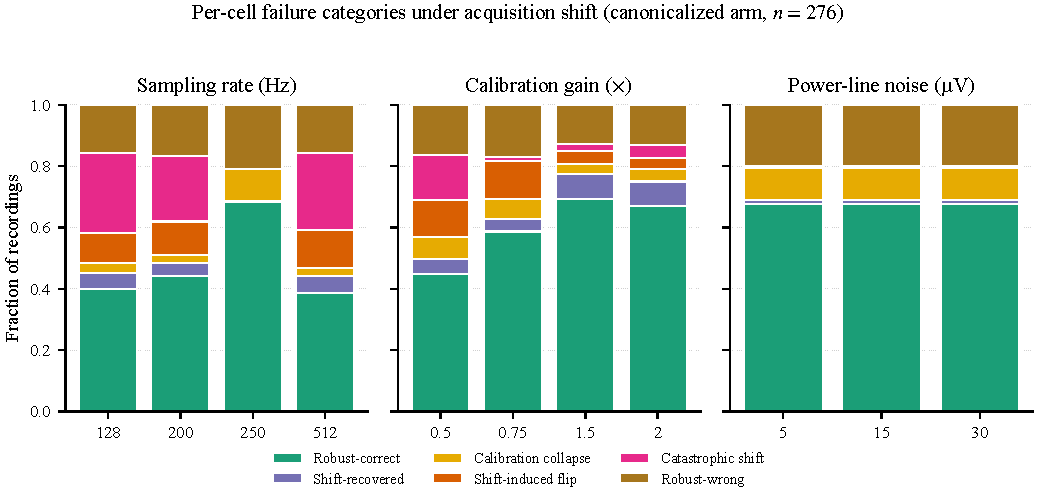
\includegraphics[width=\linewidth]{figures/fig_failure_taxonomy.pdf}
  \caption{Per-cell failure-category composition across (axis, severity) for the canonicalized arm, $n{=}276$ recordings. The \emph{catastrophic-shift} fraction (magenta) grows with sampling-rate departure from $256$\,Hz and with calibration-gain departure from $1.0\times$; canonicalized power-line filtering keeps the power-line axis near baseline. The near-absence of \emph{calibration collapse} (yellow) shows that the EEGPT-derived classifier does not equivocate under shift --- it commits with high confidence, often in the wrong direction.}
  \label{fig:failure-taxonomy}
\end{figure}

